\documentclass[12pt, letterpaper]{article}
\usepackage{graphicx}
\graphicspath{ {./} }
\usepackage[utf8]{inputenc}
\title{CS 3516 Lab 2}
\author{Joseph Petitti}
\author{jppetitti}
\date{\today}

\begin{document}

\maketitle

\begin{enumerate}
	\item IP address of www.aiit.or.kr: 58.229.6.225
	\item Authoritative DNS servers for Oxford University: ecsu-sv26.easternct.edu
	\item The IP address of the DNS server is 209.244.0.3.
	\item DNS queries and responses are sent over UDP
	\item Destination port for DNS query: 53. Source port of response: 53
	\item The DNS query message was sent to 192.168.1.1. This is the same as the address of my local DNS server (and is also the IP address of my router).
	\item This query is Type A. The query does not contain any answers.
	\item The response contains one answer, containing an IP address matched with a host name, along with a type, class, time to live, and data length.
	\item Yes, this TCP SYN packet is sent from my host to the IP address returned in the DNS query response.
	\item No, it doesn't need to issue a new DNS query because it already knows the IP address.
	\item Destination port for the DNS query message: 53. Source port for the response: 53
	\item The DNS query is sent to 192.168.1.1, which is the IP address of my default local DNS server
	\item The query is of type A and does not contain any answers.
	\item The response contains three answers, of type CNAME and A, and the canonical names and IP addresses they correspond to.
	\item See screenshot1.png

		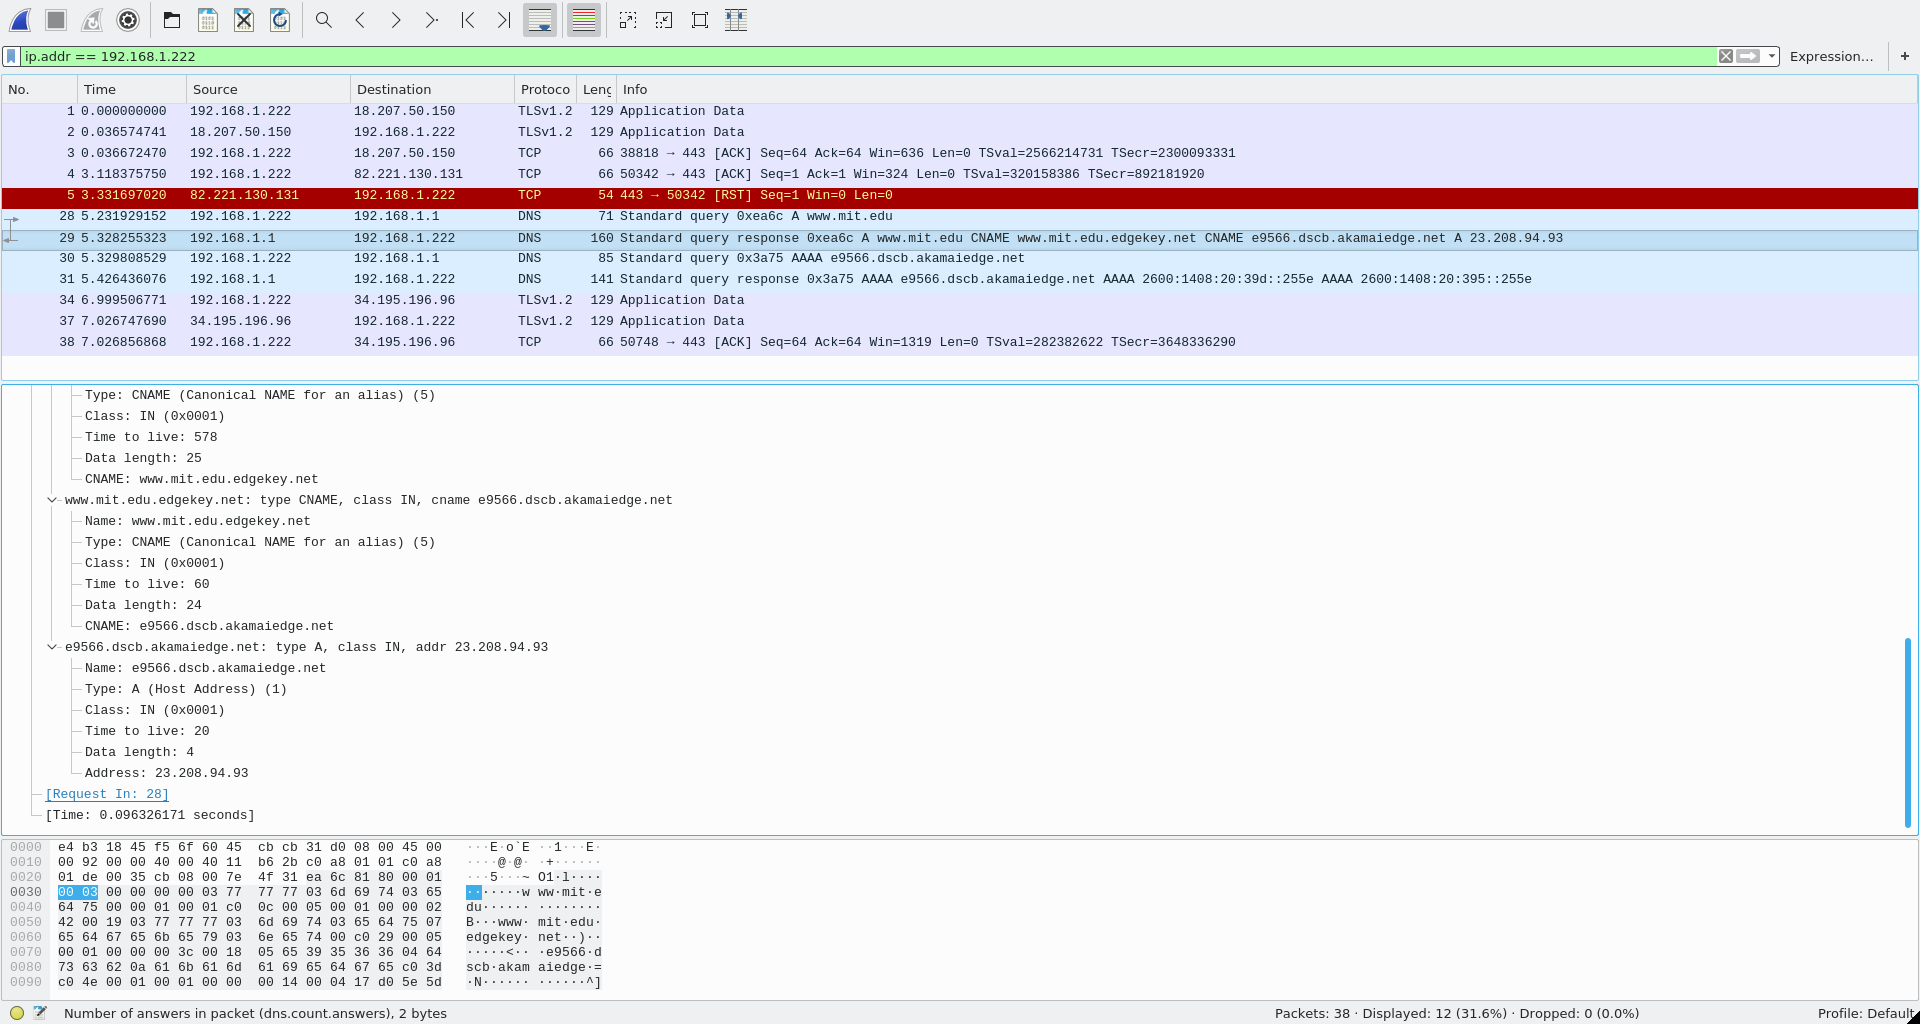
\includegraphics[width=\textwidth]{screenshot1.png}
	\item The DNS query message is sent to 192.168.1.1. This is the address of my default local DNS server.
	\item The query is of type NS, and it does not contain any answers.
	\item The response provides these MIT nameservers:
	\begin{enumerate}
		\item asia2.akam.net
		\item use2.akam.net
		\item eur5.akam.net
		\item use5.akam.net
		\item ns1-37.akam.net
		\item asia1.akam.net
		\item ns1-173.akam.net
		\item usw2.akam.net
	\end{enumerate}
		The response also includes A records listing the IP addresses for each name server.
	\item See screenshot2.png

		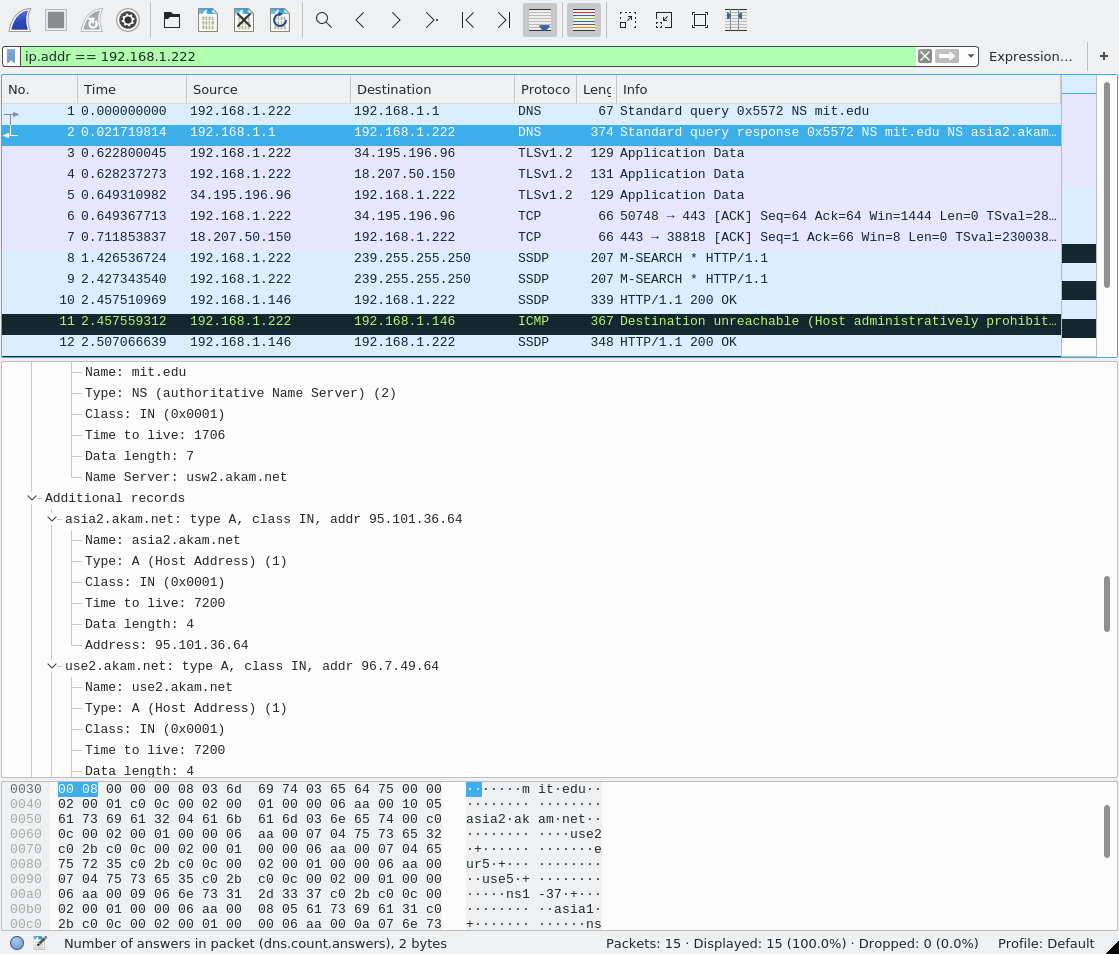
\includegraphics[width=\textwidth]{screenshot2.png}
	\item The query message is being sent to 209.244.0.3, the DNS server I specified in the command.
	\item The query message is of type A, and does not contain any answers.
	\item The DNS response message is of type A, and contains one answer, specifying a hostname and IP address pair.
	\item See screenshot3.png

		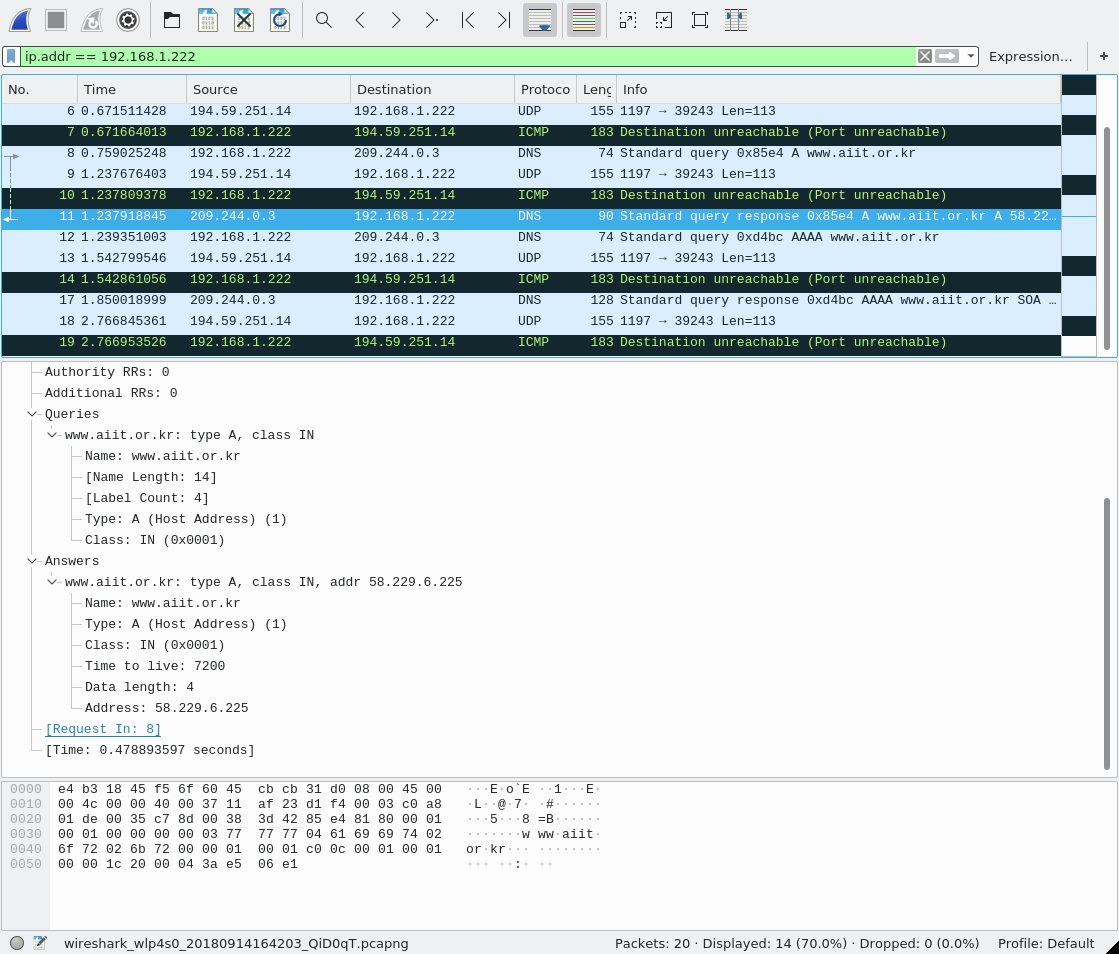
\includegraphics[width=\textwidth]{screenshot3.png}
\end{enumerate}





\end{document}
